\subsection{}
\underline{Demand and supply through a new lens}
\par
Demand is a proxy for value. The more you are willing to pay for a good, the more you value it.\\
Supply is a proxy for cost. As long as price covers cost of production, suppliers are willing to produce.\\
Therefore, equilibrium is balancing the value and cost.
\par
The triangle to the left of the equilibrium benefits economic wellbeing. 
It is called total surplus. As a measure of efficiency.
\newline
\begin{figure}[H]
    \centering
    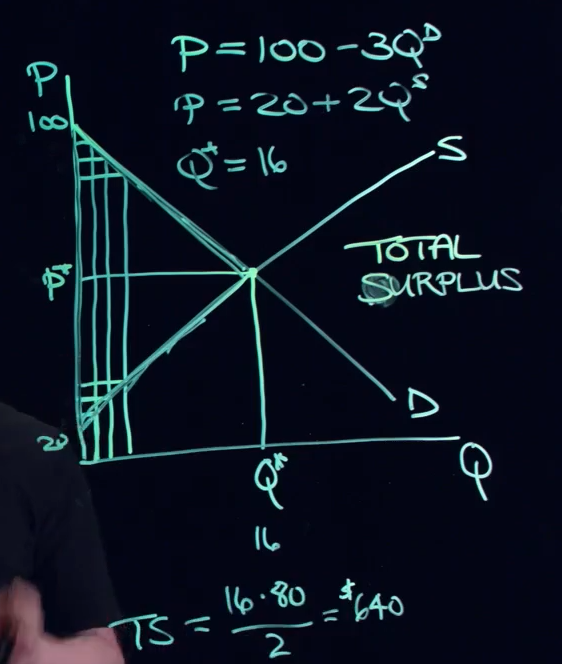
\includegraphics[width=0.5\textwidth]{Chapter5/TotalSurplus.png}
    \caption{Total Surplus}
\end{figure}
Quota is an example of \emph{Quantity Control}. It is a limit on the quantity of a good that can be produced or sold.
\par
The optimal price and quantity control is no price and quantity control.
